What do we have to do?

The user specifies some type constructors. 

'a List = Nil $|$ Cons 'a ('a List) 

this can be understood as a fixed point equations on types:

$X = 1 + A \times X$

the (co)induction package has to derive appropriate theorems for such an equation in a sound way according to the  kernel. So we formulate the following questions:

1. Given such a user definition, how do we derive the functorial 
structure?

2. Given the functorial structure, how do we derive in the logic the
induction and coinduction principles? Introduction rules? Case analysis?
And so on...This is answer by Traytel's AFP entry.

3. How could Stainless produce such (co)inductive principles?

\subsection{Functorial structure}

HOL can be modeled as a category using the universe of types $U$ as objects and functions between types as morphisms. Some useful type constructor $(\alpha_1,\ldots,\alpha_n)F$ correspond then to the notion of functor on $U$. We will rephrase the definition of functor in this context as follows:

\begin{definition}[Type constructors as functors]
	Let $\overline{\alpha}F$ be a type constructor and: $$\text{Fmap}: \overline{\alpha} \to \overline{\beta} \to \overline{\alpha} F \to \overline{\beta} F$$ be a mapping satisfying: 
	
	\begin{itemize}
		\item $\text{Fmap} \; \text{id} = \text{id}$
		\item $\text{Fmap} (\overline{g} \circ \overline{f}) = \text{Fmap} \, \overline{g} \circ \text{Fmap} \, \overline{f}$
	\end{itemize}
	
	Then we say that $(\text{F}, \text{Fmap})$ is a functor whose action on objects is $\text{F}$ and on morphisms is $\text{Fmap}$.
\end{definition}

In Isabelle, (co)datatypes are obtained composing the following basic functors:

\begin{table}[h]
	\begin{center}
		\begin{tabular}{ | l | c | r | }
			\hline
			Name & On objects & On morphisms \\ \hline
			Constant & $C_{\alpha} = \alpha$ & $\text{Cmap}_{\alpha} = id_{\alpha}$  \\ 
			Sum & $+(\alpha_1,\alpha_2) = \alpha_1 + \alpha_2$ & $f_1 \oplus f_2(\text{Inj}_i a) = \text{Inj}_i (f_i \, a)$ \\
			Product & $\times(\alpha_1,\alpha_2) = \alpha_1 \times \alpha_2$ & $f_1 \otimes f_2(x,y) = (f_1(x),f_2(y))$ \\
			Function space & $\text{func}_{\alpha}(\beta) = \alpha \to \beta$ & $\text{comp}_{\alpha} \, f \, (g) = f \circ g$ \\ 
			Powertype & $\text{set}(\alpha) = \alpha \, \text{set}$ & $\text{image}(f)(A) = f(A)$ \\ 
			k-Powertype & $\text{set}_k(\alpha) = \text{typeof } \{A: \alpha \, \text{set}. \text{card}(A) < k\}$ & $\text{image}_k = \text{image} \, f|_{\{A: \alpha \, \text{set}. \text{card}(A) < k\}}$ \\ 
			\hline
		\end{tabular}
	\end{center}
	\caption{Basic functors}
	\label{table:1}
\end{table}

Let's observe how the notion of subalgebra is simplified in this context. Let $(A,t)$ be a $F$-subalgebra of the algebra $(B,s)$. This means that the inclusion $i: A \to B$ is an $F$-algebra homomorphism. In this setting, we can actually state that $F(i) = i$. This simplifies the subalgebra equation to $s \circ i = i \circ t$ which implies that $t = s|_{F(A)}$. 

Here are some examples of the encoding of (co)datatypes using basic functors:

\begin{table}[h]
	\begin{adjustwidth}{-2.5cm}{}
		\begin{center}
			\begin{tabular}{ | l | c | c | c | r | }
				\hline
				Datatype & On objects & On morphisms & (Co)algebra structure & Abstract interface \\ \hline
				Finite lists & $(\alpha,\beta) \text{F} = \text{unit} + \alpha \times \beta$ & $\text{Fmap} \, f \, g = \text{id} \oplus f \otimes g$ & $\text{fld} = \langle \text{Nil}, \text{Cons} \rangle$ & $(\text{list},\text{map})$  \\ 
				FBFD trees & $(\alpha,\beta)F = \alpha \times \beta \; \text{list}$ & $\text{Gmap} \, f \, g = f \otimes \text{map} \, g$ & $\text{fold} = $ & b \\
				FBID trees & $(\alpha,\beta)F = \alpha \times \beta \; \text{list}$ & $\text{Gmap} \, f \, g = f \otimes \text{map} \, g$ & $\text{unf} = \langle \text{lab}, \text{sub} \rangle$ & b \\
				UFBPI trees & $(\alpha,\beta)H = \alpha \times \beta \, \text{fset}$ & $\text{Hmap} \, f \, g = f \otimes \text{fimage} \, g$ & $\text{unf} =$ & d \\
				\hline
			\end{tabular}
		\end{center}
	\end{adjustwidth}
	\caption{Examples of datatypes}
	\label{table:1}
\end{table}

The notion of bounded natural functor, provides the necessary axioms allowing to introduce initial and final coalgebras in HOL:

\begin{definition}[BNF]
	An n-ary bounded natural functor is a tuple $($F, Fmap, Fset, Fbd$)$ where:
	
	\begin{itemize}
		\item $F$ is an n-ary type constructor.
		\item $\text{Fmap}: \overline{\alpha} \to \overline{\beta} \to \overline{\alpha} F \to \overline{\beta} F$
		\item $\forall i \in \{1,\ldots,n\}.$ Fset$_i: \overline{\alpha}F \to \alpha_i \text{ set}$
		\item Fbd is an infinite cardinal number.
	\end{itemize}
	
	satisfying the following:
	
	\begin{itemize}
		\item (F,Fmap) is a binary functor.
		\item Fset$_i: \overline{\alpha}F \to \alpha_i \text{ set}$ is a natural transformation from:
		
		$((\alpha_1,\ldots,\alpha_{i-1},\textunderscore,\alpha_{i+1},\ldots,\alpha_n)F, \text{Fmap})$ to $(\text{set}, \text{image})$.
		\item (F,Fmap) preserves weak pullbacks.
		\item $\forall a \in \text{Fset}_i \, x,  i \in \{1,\ldots,n\}. f_i \, a = g_i \, a \implies \text{Fmap} \, \overline{f} \, x = \text{Fmap} \, \overline{g} \, x$
		\item The following cardinal bound conditions hold:
		
		$\forall x : \overline{\alpha} F, i \in {1,\ldots,n}. |\text{Fset}_i \, x | \le \text{Fbd}$
	\end{itemize}
\end{definition}

The naturality condition generalizes our observation about subalgebras for basic functors to any bounded natural functor. For a BNF, a subalgebra consists of a subset together with a restriction of the structure mapping to the substructure obtained after applying the functor to the subset. This is the so-called shape and content intuition that the authors write in their papers.

\begin{table}[h]
	\begin{adjustwidth}{-2.5cm}{}
		\begin{center}
			\begin{tabular}{ | l | c | r | }
				\hline
				F & Fset & Fbd \\ \hline
				$C_{\alpha}$ & & $\aleph_0$ \\
				$+$ &  & $\aleph_0$ \\
				$\times$ &  & $\aleph_0$ \\
				func$_{\alpha}$ & image g $U_{\alpha}$ & $\max\{|\alpha|,\aleph_0\}$  \\
				set$_k$ & & max$\{k,\aleph_0\}$ \\
				\hline
			\end{tabular}
		\end{center}
	\end{adjustwidth}
	\caption{Examples of BNF's}
	\label{table:1}
\end{table}

The set functor falls from this list since it lacks the necessary infinite bound. 

\subsection{How to derive the functorial structure?}





The user specification can be easily seen as specifying a set of recursive equations:

$\tau = \text{unit} + \alpha \times \tau$

we will omit how does one check that the right hand side is actually a functor of the above class and will focus on the following section in the construction of initial algebras and final coalgebras with an example. 


How is the map interface derived? 



\subsection{How to derive the (co)inductive principles?}

In what follows we assume that we have a bounded natural functor $F$ and describe how the corresponding (co)datatypes are encoded and (co)inductive principles derived. In particular, we will focus in solving the following system of equations:

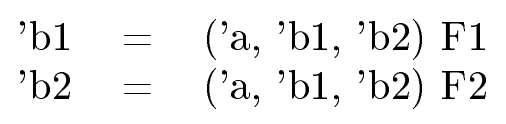
\includegraphics[width=0.3\textwidth]{img/equations.png}

\subsubsection{Encoding $F$-algebras}

Representation of algebras:

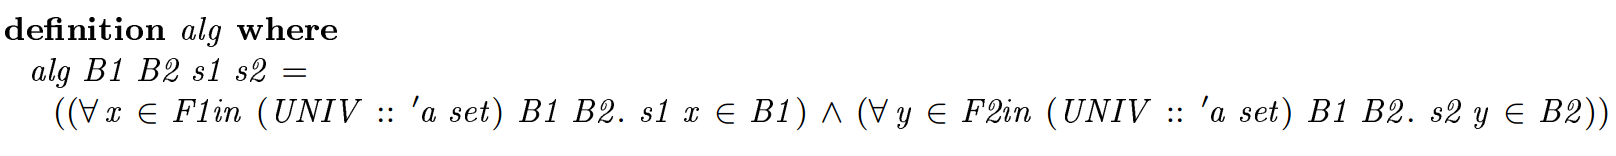
\includegraphics[width=\textwidth]{img/algebras.png}

Given morphisms $s_1: ('a, 'b, 'c) F1 \Rightarrow 'b$ and $s_2:  ('a, 'b, 'c) F2 \Rightarrow 'c$, we need to ensure that they act like structure maps on the $F$-algebra structure whose carrier set is $(B_1,B_2)$. The function Fin allows to lift from a set $S$ to the set of elements that can be built from this set using functor $S$, $F(S)$. Thus, the definition ensures that the morphisms are well-defined structure maps. 

Similarly, if one wants to specify a homomorphism $(f,g)$ between $F$-algebras $((B_1,B_2), (s_1,s_2))$ and $((B_1',B_2'), (s_1',s_2'))$ one imposes the well-definition condition on the carrier sets together with the commutativity conditions:

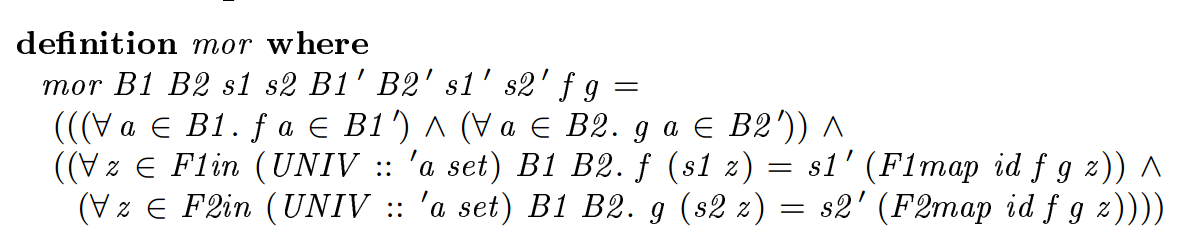
\includegraphics[width=0.7\textwidth]{img/morphisms.png}

The construction of the initial algebra happens in two stages. First one constructs  a weakly initial algebra. Then, one constructs the initial algebra from the weakly initial one. The authors systematically introduce the second step of the construction using a construction \textit{from above} of the minimal algebra generated by $\emptyset$, to then implement a construction from below that is less intuitive since it uses transfinite induction. We comment the abstract construction to precise its meaning using the remarks on subalgebras in the BNF settings that we did in the previous section. \\


\begin{construction}[Minimal algebra]
	Let $\mathcal{A}=(A,s)$ be an $F$-algebra. Set $M_s = \bigcap_{B. (B,s) \text{is a subalgebra of (A,s)}} B$ then: \[
	\mathcal{M}(\mathcal{A}) = \Big(M_s,s \Big|_{M_s} \Big)\]
	
	is the $F$-subalgebra generated by $\emptyset$.
\end{construction}	

For a formal proof that the intersection of subalgebras of a general $F$-algebra is again a subalgebra, the interested reader is referred to \cite{denecke2009universal} (theorem 5.6.5) which provides a good mathematical account of the subject. $\mathcal{A}$ is said to be the subalgebra generated by $\emptyset$ in the sense that it is the intersection of all subalgebras containing $\emptyset$. \\
	
\begin{lemma}\label{lem}
	There exists at most one morphism from $\mathcal{M}(\mathcal{A})$ to any other $F$-algebra $(Y,t)$.
\end{lemma}	
\begin{proof}
	If $f,g$ are two such morphisms, we can show that: $$B = \mathcal{M}(\mathcal{A}) \cap \{x \in \mathcal{A}. f(x) _= g(x)\}$$ is a $F$-subalgebra of $\mathcal{A}=(A,s)$
	
	Indeed, by our remarks, it suffices to note that $M_s \cap \{x \in \mathcal{A}. f(x) _= g(x)\} \subseteq M_s$ and consider the structure map $s|_B$. This leads to a subalgebra of $\mathcal{M}(\mathcal{A})$ which can be naturally seen as a subalgebra of $\mathcal{A}$. 
	
	By definition of $\mathcal{M}(\mathcal{A})$, $M_s \supseteq B$ and thus $\forall x \in M_s. f(x) = g(x)$. Thus, the morphisms are equal. 
\end{proof}
	
Here is the naive approach to the construction of an initial $F$-algebra.

\begin{enumerate}
	\item Set $\mathcal{R} = \prod \{\mathcal{A}. \mathcal{A} \text{ is an algebra}\}$.
	\item Given an algebra $\mathcal{A}$, note $h$ the projection morphism from $\mathcal{R}$ to $\mathcal{A}$.
	\item Then $h|_{\mathcal{M}(\mathcal{R})}$ is the unique morphism between $\mathcal{M}(\mathcal{R})$ and $\mathcal{A}$.
	\item Since the construction does not depend on the chosen algebra $\mathcal{A}$,  $\mathcal{M}(\mathcal{R})$ is the desired initial algebra.
\end{enumerate}

The naive approach cannot be encoded in HOL. First, one cannot quantify over infinite type collections. Second, the product of the carrier sets of all algebras, fails itself to be a set. 

Here is the enhanced naive approach to the construction of an initial $F$-algebra. Essentially, we split the construction in two phases:

Given an $F$-algebra $\mathcal{A}$ we know that there exists at most one morphism $\mathcal{M}(\mathcal{A}) \to \mathcal{A}$. But from our remarks above, for bounded natural functors, the inclusion is one such morphism. So there is exactly one morphism $g: \mathcal{M}(\mathcal{A}) \to \mathcal{A}$.

On the other hand, we would like some set of algebras $\mathcal{R}$ such that from $\mathcal{R}$ there is a unique morphism to any $\mathcal{M}(\mathcal{A})$. The strategy is two find a sufficiently large type $T_0$ such that its cardinality is an upperbound for any $\mathcal{A}$. The reason is a theorem stating that if we can bound the cardinality of a set by some ordinal then the set has a bijective representation on the carrier of the wellorder inducing the ordinal. The crucial lemma is ex\_bij\_betw:

$|A| \le_o (r :: 'b \, \text{set}) \implies \exists f \; B::'b \; \text{set}. \text{bij\_betw} f \; B \; A$

More precisely, the package shows that for all algebras $\mathcal{A}$, if $M$ denotes the carrier of $\mathcal{M}(\mathcal{A})$ then $|M| \le_o 2  \wedge_c k$. Then, the package witnesses a type $T_0$ with this cardinality and defines $\mathcal{R} = \prod \{\mathcal{A}. \mathcal{A} = (A,s) \text{ is an algebra with structure map } s: T_0 F \to T_0 \}$. By means of $ex\_bij\_betw$ the minimal algebras $\mathcal{M}(\mathcal{A})$ have isomorphic representants on a component of $\mathcal{R}$. Thus, the corresponding projection from the product to $\mathcal{M}(\mathcal{A})$ restricted to $\mathcal{M}(\mathcal{R})$ is the unique morphism  $f$ between the two. 

Then, $f \circ g: \mathcal{M}(\mathcal{R}) \to \mathcal{A}$ is a suitable morphism. One shows it is the unique morphism between the two with a similar argument as in lemma \ref{lem}.

It should be noted that the real proof does not even define $\mathcal{M}(\mathcal{A})$ as we did. Instead, the underlying construction defines the minimal algebra from below using transfinite recursion.

\subsubsection{Derived theorems and definitional framework for datatypes}

Once we understand the way in which one could compute an initial algebra of a functor, it is time to encode the proving and definitional tools that this theoretical object provides us. First we formulate the general induction principle obtained:

\begin{thm}[Induction principle of a BNF]
	Let $(\varphi_1,\dots,\varphi_n): (\overline{\alpha} IF^1,\ldots,\overline{\alpha} IF^n) \to bool$ be a tuple of predicates. Then:
	
	\[
	\infer{\forall b_1,\ldots,b_n. \varphi_1(b_1) \land \ldots \land \varphi_n(b_n)}{%
		\forall y. \forall j \in \{1,\ldots,n\}. (\bigwedge_{k = 1}^n \forall b \in \text{Fset}_{m+k}^j y. \varphi_k(b)) \implies \varphi_j(\text{fld}^j(y))
	}
	\]
\end{thm}

The package also defines iterator $iter^j$ and recursor $rec^j$ constants in a way that the following diagrams commute for each $j \in \{1,\ldots\}$. 

\begin{tikzcd}
	(\overline{\alpha},\overline{\alpha} IF^1,\ldots,\overline{\alpha} IF^n)F^j \arrow{r}{fld^j} \arrow[swap]{d}{Fmap^j \; id \ldots id \; (iter^1 s_1 \ldots s_n) \ldots (iter^n s_1 \ldots s_n)} 
	& \overline{\alpha} IF^j \arrow{d}{iter^ j s_1 \ldots s_n} \\
	(\overline{\alpha},\beta_1,\ldots,\beta_n)F^j \arrow{r}{s_j}  & \beta_j
\end{tikzcd}

\begin{tikzcd}
	(\overline{\alpha},\overline{\alpha} IF^1,\ldots,\overline{\alpha} IF^n)F^j \arrow{r}{fld^j} \arrow[swap]{d}{Fmap^j \; id \ldots id \; \langle id, rec^1 s_1 \ldots s_n \rangle \ldots \langle id, rec^n s_1 \ldots s_n \rangle} 
	& \overline{\alpha} IF^j \arrow{d}{rec^ j s_1 \ldots s_n} \\
	(\overline{\alpha},\overline{\alpha} IF^1 \times \beta_1,\ldots,\overline{\alpha} IF^n \times \beta_n)F^j \arrow{r}{s_j}  & \beta_j
\end{tikzcd}

More importantly, all this infrastructure is used in defining the BNF corresponding to the initial algebra. This allows to compose BNF's which yields the ultimate power of categorical method: the simplicity of composing its underlying constructions.

\begin{thm}
	$(IF^ j, IFmap^ j, IFset^ j, IFbd)$ defined for $j \in \{1,\ldots,n\}$ as:
	
	\begin{itemize}
		\item $\overline{\alpha} \, IF^j$ is the set constructed in the previous section.
		\item $IFmap^j: (\overline{\alpha} \to \overline{\beta}) \to (\overline{\alpha} IF^j \to \overline{\beta} IF^j)$ \\
			  $IFmap^j \, f_1 \, \ldots \, f_m = iter^j (fld^1 \circ Fmap^1 f_1 \ldots f_m \, id \ldots id) \ldots (fld^ n \circ Fmap^ n f_1 \ldots f_m \, id \ldots id)$
		\item $IFset_i^j: \overline{\alpha} \, IF^j \to \alpha_i \, set, i \in \{1,\ldots,m\}$ \\
			  $IFset_i^j = iter \, (\lambda z. Fset_i^1 z \cup \bigcup_{k=m+1}^{m+n} \cup Fset_k^1 z) \ldots (\lambda z. Fset_i^n z \cup \bigcup_{k=m+1}^{m+n} \cup Fset_k^n z)$ 
		\item $IFbd = 2^{\max\{Fbd^1,\ldots,Fbd^n\}}$
	\end{itemize}

is a BNF.
\end{thm}

Here $m$ is a parameter ensuring that the different equations share the same variables. The first $m$ occurrences are considered dead and do not play a role in this section, thus the increment by $m$ in the above formula. Also, $n$ tells the number of involved equations.

For the definition of $IFset$, we focus on the first equation:

$collect_i = \lambda z. Fset_i^1 z \cup \bigcup_{k=m+1}^{m+n} \cup Fset_k^1 z$ 

this function allows to compute the atoms of type $\alpha_i$ and then 

In the first union, we add the atoms of that variable type regardless of if it is live or not, in the rest of the union we add the atoms of the inductive components.


\begin{example}[BNF structure of lists]
	Let's see how the construction for $IFmap$ works on lists of base type $\alpha$. If we set $(\alpha,\beta)F = unit + \alpha \times \beta \, list$ then we have:

\begin{tikzcd}
	(\alpha,\alpha \, list) \arrow{r}{F(iter(s))} \arrow[swap]{d}{fld_{\alpha}} & (\alpha, \beta \, list)F \arrow{d}{Fmap \, f \, id} \arrow[bend left=90]{dd}{s} \\
	\alpha \, list \arrow[dashed,swap]{rd}{iter(s)} & (\beta, \beta \, list)F \arrow{d}{fld_{\beta}} \\
	& \beta list                                   
\end{tikzcd}


and our map function is $IFmap = iter(s) = iter(fld_{\beta} \circ Fmap \, f \, id)$. So from the mapping registered in the system there is a way to give the abstract interface $(list,map)$ of lists. 

The atoms of type $\beta$ are obtained with $Fset_1$ while onje delves into the inductive components by means of $Fset_2$:

\begin{tikzcd}
	(\beta,\beta \, IF)F \arrow[swap]{d}{fld} \arrow{r}{Fmap \, id \, IFset} &  (\beta, \beta \, set)F  \arrow{d}{collect} \\
	\beta \, IF \arrow{r}{IFset}  & \beta \, set                       
\end{tikzcd}

where $collect(a) = Fset_1(a) \cup Fset_2(a)$ and $IFset$ is defined by $IFset = iter(collect)$. 
\end{example}


\subsubsection{Encoding $F$-coalgebras}

Coge un tipo de dato coinductivo.
Formulalo como un functor.
Sigue las pruebas en GFP.

\subsubsection{Derived theorems and definitional framework for codatatypes}


\subsection{How could Stainless produce such (co)inductive principles?}

See section 2.4.4 of Jacobs coalgebras for a way of emulating coalgebras using artificial constructions. Stainless does it in a way similar to Coq with some abstract mechanism to deal with them.  

See also the images on the topic on the coinduction files under images. For the Stainless approach. 


\subsection{Basic natural functors}

Our objects are types from a type universe $U$. 

These are described theoretically in chapter 3 of \cite{traytel}. Let us take the example of the sum functor:



In /src/HOL/Tools/BNF/bnf\_def.ML we can see the definition of a bounded natural functor:

\begin{lstlisting}
	datatype bnf = BNF of {
		name: binding,
		T: typ,
		live: int,
		lives: typ list, (*source type variables of map*)
		lives': typ list, (*target type variables of map*)
		dead: int,
		deads: typ list,
		map: term,
		sets: term list,
		bd: term,
		axioms: axioms,
		defs: defs,
		facts: facts,
		nwits: int,
		wits: nonemptiness_witness list,
		rel: term,
		pred: term
	};
\end{lstlisting}

as a datatype constructor with only one sort which takes a record as a parameter. 

Some examples of how to build and proof a BNF correct can be found in /src/HOL/Basic\_BNFs.thy


Construction of an initial algebra from a weakly initial algebra

Let $\mathcal{A} = (A,s)$ be an algebra.

Let $M_s$ be the intersection of all sets $B$ such that $(B,s)$ is an algebra.

It seems evident that if we understand the minimal algebra generated by $\mathcal{A}$, $M(\mathcal{A})$ as a subalgebra, such that any other subalgebra is a subalgebra of this one.

Statement 1: $\mathcal{M}(\mathcal{A}) = (M_s,s)$

Statement 2: there exists at most one morphism from $M(\mathcal{A})$ to any other algebra...

Statement 3: given a weakly initial algebra $\mathcal{C}$, the desired initial algebra is its minimal subalgebra $\mathcal{M}(\mathcal{C})$ 